\documentclass[aspectratio=43]{beamer}
% Theme works only with a 4:3 aspect ratio
\usetheme{CSCS}

\usepackage{tikz}
\usepackage{pgfplots}
\usepackage{pgfplotstable}
\usetikzlibrary{pgfplots.groupplots,spy,patterns}
\usepackage{listings}
\usepackage{color}
\usepackage{tcolorbox}
\usepackage{anyfontsize}
\usepackage{xspace}
\usepackage{graphicx}

% define footer text
\newcommand{\footlinetext}{Introduction to GPUs in HPC}

% Select the image for the title page
\newcommand{\picturetitle}{cscs_images/image5.pdf}

% fonts for maths
\usefonttheme{professionalfonts}
\usefonttheme{serif}

% source code listing
\newcommand{\axpy}{{\ttfamily axpy}\xspace}

% set indent to a more reasonable level (so that itemize can be used in columns)
\setlength{\leftmargini}{20pt}

\DeclareTextFontCommand{\emph}{\bfseries\color{blue!70!black}}

% Please use the predifined colors:
% cscsred, cscsgrey, cscsgreen, cscsblue, cscsbrown, cscspurple, cscsyellow, cscsblack, cscswhite

\author{Ben Cumming, CSCS}
\title{Introduction to GPUs in HPC\\CSCS Summer School 2020}
\subtitle{}
\date{\today}

\begin{document}

% TITLE SLIDE
\cscstitle

\cscschapter{Introduction}

%%%%%%%%%%%%%%%%%%%%%%%%%%%%%%%%%%%%
\begin{frame}[fragile]{Course Overview}
%%%%%%%%%%%%%%%%%%%%%%%%%%%%%%%%%%%%
    Over these two days we will cover a range of topics:
    \begin{itemize}
        \item Learn about the GPU memory model;
        \item Implement parallel CUDA kernels for simple linear algebra;
        \item Learn how to scale our parallel kernels to utilize all resources on the GPU;
        \item Learn about thread cooperation and synchronization;
        \item Learn about concurrent task-based parallelism;
        \item Learn how to profile GPU applications.
        \item Port the miniapp to the GPU.
    \end{itemize}
\end{frame}

%%%%%%%%%%%%%%%%%%%%%%%%%%%%%%%%%%%%
\begin{frame}[fragile]{Course Overview}
%%%%%%%%%%%%%%%%%%%%%%%%%%%%%%%%%%%%
    We focus on HPC and modern GPU architectures, specifically:
    \begin{itemize}
        \item HPC development for P100 GPUs on Piz Daint;
        \item Using CUDA toolkit version 10 and above;
        \item Some are available on P100 and later GPUs.
        \begin{itemize}
            \item  e.g. double precision atomics.
        \end{itemize}
        \item Likewise, we won't be covering some features that are available on the latest ``Volta'' GPUs.
    \end{itemize}
\end{frame}

%%%%%%%%%%%%%%%%%%%%%%%%%%%%%%%%%%%%
\begin{frame}[fragile]{Course Overview}
%%%%%%%%%%%%%%%%%%%%%%%%%%%%%%%%%%%%
    There aren't many prerequisites for the course:
    \begin{itemize}
        \item No GPU or graphics experience required.
        \item I assume C++11 knowledge.
        \item The generic GPU programming concepts from CUDA are useful for when:
        \begin{itemize}
            \item Developing with OpenACC, OpenCL and GPU-ready libraries.
            \item Using ML frameworks that use GPU for compute.
        \end{itemize}
    \end{itemize}
\end{frame}

%++++++++++++++++++++++++++++++++
\cscschapter{Why GPUs?}
%++++++++++++++++++++++++++++++++

%%%%%%%%%%%%%%%%%%%%%%%%%%%%%%%%%%%%
\begin{frame}[fragile]{}
%%%%%%%%%%%%%%%%%%%%%%%%%%%%%%%%%%%%
    \begin{info}{There is a trend towards more parallelism ``on node''}
        \emph{Multi-core CPUs} get more cores and wider vector lanes:
        \begin{itemize}
            \item 24-core$\times$SMT 4$\times$SIMD 128: IBM Power9 (2017).
            \item 28-core$\times$SMT 2$\times$SIMD 512: Intel Xeon (2020);
            \item 48-core$\times$SMT 1$\times$SIMD 512: Fujitsu ARM A64FX (2020).
        \end{itemize}
        \emph{Many-core Accelerators} with many highly-specialized cores and high-bandwidth memory:
        \begin{itemize}
            \item NVIDIA P100 GPUs with 3584 cores (2016);
            \item NVIDIA V100 GPUs with 5120 cores (2017);
            \item NVIDIA A100 GPUs with 8192 cores (2020).
        \end{itemize}
    \end{info}

\end{frame}

%%%%%%%%%%%%%%%%%%%%%%%%%%%%%%%%%%%%
\begin{frame}[fragile]{A Piz Daint node}
%%%%%%%%%%%%%%%%%%%%%%%%%%%%%%%%%%%%
    \begin{center}
        \includegraphics[width=1\textwidth]{./images/node.pdf}
    \end{center}
    \dots that is a lot of parallelism!
\end{frame}


%%%%%%%%%%%%%%%%%%%%%%%%%%%%%%%%%%%%
\begin{frame}[fragile]{MPI and the free lunch}
%%%%%%%%%%%%%%%%%%%%%%%%%%%%%%%%%%%%
    HPC applications were ported to use the message passing library MPI in the late 90s and early 2000s at great cost and effort
    \begin{itemize}
        \item Individual nodes with one or two CPUs
        \item Break problem into chunks/sub-domains
        \item Explicit message passing between sub-domains
    \end{itemize}
    The ``free lunch'' was the regular speedup in codes as CPU clock frequencies increased and as the number of nodes in systems increased
    \begin{itemize}
        \item With little/no effort, each new generation of processor bought significant speedups.
    \end{itemize}

    \dots  but there is no such thing as a free lunch.
\end{frame}

%%%%%%%%%%%%%%%%%%%%%%%%%%%%%%%%%%%%
\begin{frame}[fragile]{}
%%%%%%%%%%%%%%%%%%%%%%%%%%%%%%%%%%%%
    \begin{center}
        \includegraphics[width=\textwidth]{./images/transistors.pdf}

        The number of transistors in processors has increased exponentially for 45 years.
    \end{center}
\end{frame}

%%%%%%%%%%%%%%%%%%%%%%%%%%%%%%%%%%%%
\begin{frame}[fragile]{}
%%%%%%%%%%%%%%%%%%%%%%%%%%%%%%%%%%%%
    \begin{center}
        \includegraphics[width=\textwidth]{./images/fp-perf.pdf}

        Floating point performance per core is not keeping up \dots
    \end{center}
\end{frame}

%%%%%%%%%%%%%%%%%%%%%%%%%%%%%%%%%%%%
\begin{frame}[fragile]{}
%%%%%%%%%%%%%%%%%%%%%%%%%%%%%%%%%%%%
    \begin{center}
        \includegraphics[width=\textwidth]{./images/frequency.pdf}

        Clock speeds peaked around 2005.

        \textbf{The problem}: power $\propto$ frequency$^3$
    \end{center}
\end{frame}

%%%%%%%%%%%%%%%%%%%%%%%%%%%%%%%%%%%%
\begin{frame}[fragile]{How to speed up an application}
%%%%%%%%%%%%%%%%%%%%%%%%%%%%%%%%%%%%
    There are 3 ways to increase performance:
    \begin{enumerate}
        \item Increase clock speed.
        \item Increase the number of operations per clock cycle:
        \begin{itemize}
            \item vectorization;
            \item instruction level parallelelism;
            \item more cores.
        \end{itemize}
        \item Don't stall:
        \begin{itemize}
            \item e.g. cache to avoid waiting on memory requests;
            \item e.g. branch prediction to avoid pipeline stalls.
        \end{itemize}
    \end{enumerate}
\end{frame}

%%%%%%%%%%%%%%%%%%%%%%%%%%%%%%%%%%%%
\begin{frame}[fragile]{Clock frequency won't increase}
%%%%%%%%%%%%%%%%%%%%%%%%%%%%%%%%%%%%
    In fact, clock frequencies have been going down as the number of cores increases:
    \begin{itemize}
        \item A 4-core Haswell processor at 3.5 GHz (4*3.5=14 Gops/second) has the same power consumption as a 12-core Haswell at 2.6 GHz (12*2.6=31 Gops/second);
        \item A P100 GPU with 3584 CUDA cores runs at 1.1 GHz.
    \end{itemize}

    \begin{info}{Caveat}
        It is not reasonable to compare a CUDA core and an X86 core.
    \end{info}
\end{frame}

%%%%%%%%%%%%%%%%%%%%%%%%%%%%%%%%%%%%
\begin{frame}[fragile]{Parallelism will increase}
%%%%%%%%%%%%%%%%%%%%%%%%%%%%%%%%%%%%
    \begin{itemize}
        \item The number of cores in both CPUs and accelerators will continue to increase
        \item The width of vector lanes in CPUs will increase
        \begin{itemize}
            \item 8$\times$SIMD double for AVX512 and SVE (Intel and ARM).
        \end{itemize}
        \item The number of threads per core will increase
        \begin{itemize}
            \item Intel SkyLake: 2 threads/core
            \item Intel KNL: 4 threads/core
            \item IBM Power-8: 8 threads/core
        \end{itemize}
    \end{itemize}
\end{frame}

%%%%%%%%%%%%%%%%%%%%%%%%%%%%%%%%%%%%
\begin{frame}[fragile]{Memory is slow}
%%%%%%%%%%%%%%%%%%%%%%%%%%%%%%%%%%%%
    Memory is much slower than processors
    \begin{itemize}
        \item For both CPU and GPU the latency of fetching a cache-line from memory is 100s of cycles\dots
        \item \dots 100s of cycles that the processor is stalled
        \item Latency has to be hidden or reduced to minimise stalling
    \end{itemize}
\end{frame}

%%%%%%%%%%%%%%%%%%%%%%%%%%%%%%%%%%%%
\begin{frame}[fragile]{Low Latency or High Throughput?}
%%%%%%%%%%%%%%%%%%%%%%%%%%%%%%%%%%%%
    \begin{columns}[T]
        \begin{column}{0.6\textwidth}
            \emph{CPU}
            \begin{itemize}
                \item   Optimized for low-latency access to cached data sets.
                \item   Control logic for out-of-order and speculative execution.
            \end{itemize}

            \vspace{0.75cm}

            \emph{GPU}
            \begin{itemize}
                \item   Optimized for data-parallel, throughput computation.
                \item   Architecture tolerant of memory latency.
                \item   More transistors dedicated to computation.
            \end{itemize}
        \end{column}

        \begin{column}{0.4\textwidth}
            \vspace{-0.2cm}
            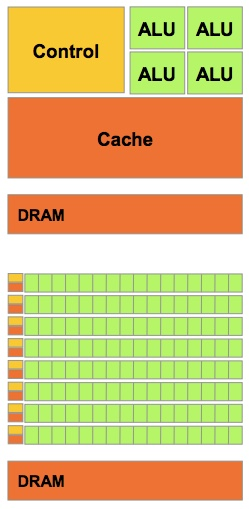
\includegraphics[width=0.8\textwidth]{./images/layout.jpg}

            \footnotesize \textcopyright NVIDIA Corporation 2010
        \end{column}
    \end{columns}
\end{frame}

%%%%%%%%%%%%%%%%%%%%%%%%%%%%%%%%%%%%
\begin{frame}[fragile]{GPUs are throughput devices}
%%%%%%%%%%%%%%%%%%%%%%%%%%%%%%%%%%%%
    \begin{itemize}
        \item CPU cores are optimized to minimize latency between operations.
        \item GPUs aim to minimize latency between operations by scheduling multiple warps (thread bundles).
    \end{itemize}
    \begin{center}
        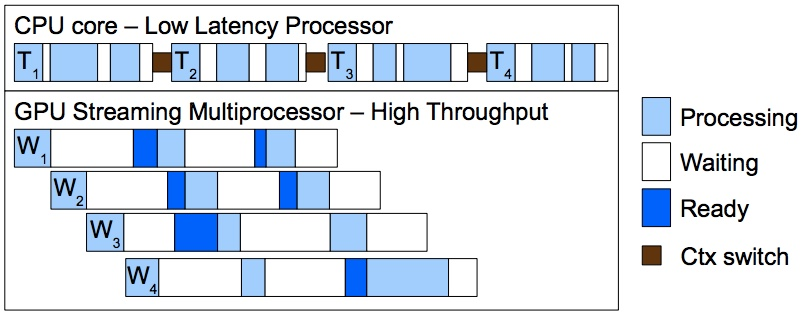
\includegraphics[width=0.8\textwidth]{./images/latency.jpg}
    \end{center}
    \footnotesize \textcopyright NVIDIA Corporation 2010
\end{frame}

%%%%%%%%%%%%%%%%%%%%%%%%%%%%%%%%%%%%
\begin{frame}[fragile]{Many applications aren't designed for many core}
%%%%%%%%%%%%%%%%%%%%%%%%%%%%%%%%%%%%
    \begin{itemize}
        \item Exposing sufficient fine-grained parallelism for multi and many core processors is hard.
        \item New programming models are required.
        \item New algorithms are required.
        \item Existing code has to be rewritten or refactored.
    \end{itemize}

    On-node parallelism will continue to increase:
    \begin{itemize}
        \item Piz Daint @ CSCS (2015): 1 GPU + 1 CPU.
        \item Marconi100 @ CINECA (2020): 4 GPU + 2 CPU.
        \item EUROHPC pre-exascale (2021): 4 GPU + 1 CPU.
        \item US ECP exascale (2021-2023): 4 GPU + 1 CPU.
    \end{itemize}
\end{frame}


%%%%%%%%%%%%%%%%%%%%%%%%%%%%%%%%%%%%
\begin{frame}[fragile]{TLDR: Change because power}
%%%%%%%%%%%%%%%%%%%%%%%%%%%%%%%%%%%%
    Writing good concurrent code for many-core is difficult
    \begin{itemize}
        \item But the days of easy speed up each generation of CPU are over
        \begin{itemize}
            \item Performance gains must not increase power consumption
        \end{itemize}
        \item This course will be about one type of many-core architecture NVIDIA GPUs
        \begin{itemize}
            \item CUDA is GPU-specific.
            \item Conceptually very close to HIP, OpenCL and SYCL (AMD/NVIDIA/Intel).
        \end{itemize}
    \end{itemize}
\end{frame}

\end{document}

